\section{Introduction}

\vspace*{1cm}

\subsection{Climate change and its impact on ecosystems}

\subsubsection{Past and current climate trends} \label{sec:climate}

The year 2023 has been recorded as the warmest year since 1850 (\href{https://climate.copernicus.eu/copernicus-2023-hottest-year-record}{copernicus.eu}; \autoref{fig:climatestate}). Apart from the extreme temperatures this can cause in a south-facing office in Montpellier, it is a striking example of the ongoing climate change. In the Northern Hemisphere, the summer was 2.07 °C warmer than the 1850-1900 instrumental mean -- and was the warmest summer over the past 2000 years \citep{Esper2024}. As the atmospheric concentrations of carbon dioxide continues to increase (reaching 419 ppm in 2023), extremes are becoming more frequent and intense -- and are at least partially induced by human-induced climate change \citep{Trenberth2015, Diffenbaugh2017}.
% even though the imapcts of extreme is still not fully understand...
These records provide a stark reminder of how drastically our current climate differs from the one in which our civilization has developed.

\begin{figure}[hp]
\hspace*{-0.8cm}
\centering
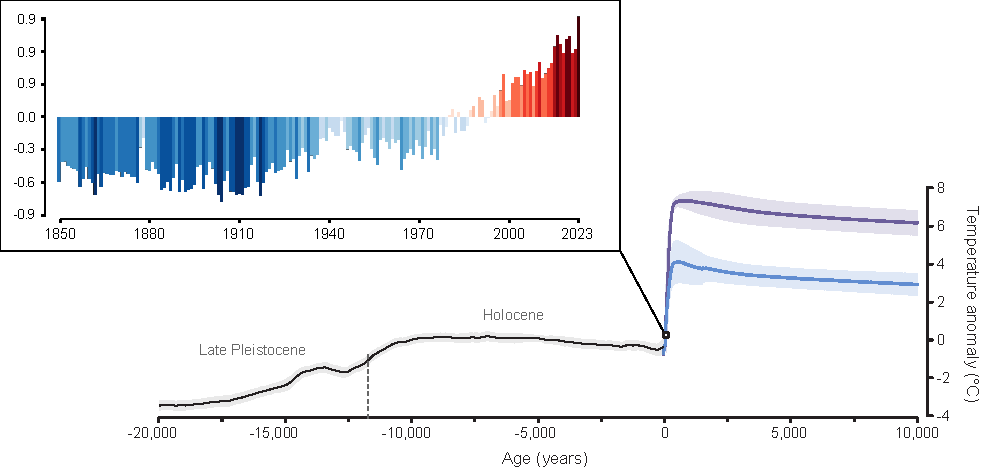
\includegraphics{0introduction/figs/clark2016_climatestrips.pdf}
\caption{\textbf{Past and future changes of global mean temperature.} The main plot is adapted from \citet{Clark2016} and shows the temperature (mean$\pm$SD) reconstructed from palaeoclimate archives for the past 20,000 years and from simulations with the UVic and Bern3D-LPX models for the next 10,000 years, for two emission scenarios (blue: 2,560 PgC, purple: 5,120 PgC). The inset plot shows the recent (1850-2023) trend according to the HadCRUT5 dataset (compiled by the UK Met Office), following the \emph{warming stripes} visualization created by \href{https://showyourstripes.info/}{Ed Hawkins}.}
\label{fig:climatestate}
\end{figure}

The study of paleoclimate indeed helps to place our understanding of the magnitude and speed of recent climate change in the context of natural climate variability \citep{IPCC2021, Tierney2020}. Thanks to proxy data (such as ice cores), we know that the Earth has alternated between warm (greenhouse periods) and cold conditions (ice ages) -- we are currently in the Quaternary glaciation which has begun 2.58 millions years ago. Throughout the Quaternary period, several glacial and interglacial cycles have occurred, triggered by slow (multi-millennial) orbital variations followed by several feedback loops (sea ice retreat, greenhouse gases; \citealp{Snyder2016, Koehler2010}).
The last major event of global warming in Earth’s history was the transition from the Last Glacial Maximum ($\sim$21,000 years ago) to the start of the interglacial period we are now experiencing (11,700 years ago; \Cref{fig:climatestate}). 
This period, called the Holocene, is characterized by warm and stable climatic conditions that have allowed human civilization to flourish (e.g. development of farming). \\
However, past climate archives also show us that, over the last 50 years, human activities have warmed the climate at a rate that is unprecedented in at least 2000 years. Many climate indicators are at levels not experienced for centuries to millennia \citep{IPCC2021}, and the climate trajectory we are currently on is already profoundly affecting many components of the biosphere.

\subsubsection{How climate change is affecting ecosystems, and vice-versa} \label{sec:forest}

Climate is a primary driver of ecosystem dynamics, and affects numerous ecological processes. Climate change impacts are already observed all over the world \citep{IPCC2021}. The ranges of many terrestrial organisms are shifting in response to global warming: species generally move towards higher latitudes and elevations, i.e. cooler conditions \citep{Lenoir2008, Elmendorf2015, Pecl2017, Vitasse2021, Rumpf2018, Zurell2024}. Notably, a meta-analysis reported a median rate of 16.9 kilometers per decade for many species, including plants, insects and birds \citep{Chen2011}. However, this poleward migration can be slower than expected for tree species \citep{Harsch2009, Renwick2015}, and other confounding factors can lead to unexpected dynamics \citep{Lawlor2024}. Phenological events are also shifting: animals are active earlier in the spring, as well as plants are blooming and leafing out earlier \citep{Vitasse2021, Fu2015, Fu2019}. This may in turn induce shifts in the synchrony of species and affect different trophic levels \citep{Kharouba2018, Beard2019}. As a result, novel communities may emerge, with novels species, interactions and functions \citep{Hobbs2009, Radeloff2015, Ordonez2024}.

% Forests in Europe
Forests are also affected by these major changes all around the globe. 
Past climate changes induced large-scale vegetation shifts \citep{Hoogakker2016, Nolan2018}, and triggered major extinctions \citep{Svenning2003}. During the Early Eocene ($\sim$52 million years ago), Arctic was even covered by dense forests inhabited by a rich vertebrate fauna \citep{Eberle2010}. During the last warming episode of the Early Holocene, trees migrated from glacial refugia to colonize previously ice-covered terrain \citep{Brewer2002, TerhuerneBerson2004,  Saltre2013} -- not only from southern Europe but also from more northern refugia \citep{Robin2016}. These past dynamics have greatly contributed to shaping the forests we know, both in terms of species diversity \citep{Svenning2007} and genetic diversity \citep{Cheddadi2006}. Today, accumulating evidences show that warmer and drier than average climate conditions are impacting forest ecosystems \citep{Allen2010, Senf2020}.  On the one hand, warmer conditions had lengthened, until recently, the growing season with advanced spring leafout and delayed leaf senescence \citep{Menzel1999}. In Europe, tree leafout was on average 10 days earlier in 2002–2016 than in 1951–1965 \citep{Fu2019}. On the other hand, increasing evapotranspiration in the last decade (2011–2020) was responsible for an earlier leaf senescence and a shorter growing season in Europe \citep{Rahmati2023}. Droughts can also trigger mortality directly (hydraulic failure; \citealp{Hartmann2018}), increase the probability of large-scale fires and induce legacy effects in surviving trees with an increased vulnerability to insect outbreaks and other pathogens \citep{Breshears2005, Seidl2017, Sommerfeld2018, Jactel2012, Mantgem2009, Hember2016}. In Europe, droughts were responsible for an excess forest mortality of 500,000 hectares between 1987 and 2016 \citep{Senf2020}. Similarly, the 2022 severe summer drought occurred in about third of the continent and decreased the forest productivity in several countries \citep{Woude2023}. Forest disturbance regimes are thus significantly changing across all forests, though with a considerable within-biome variability, notably because of the large variability in species ecophysiology \citep{Sommerfeld2018}. This global increase in tree mortality is a particular concern in Europe, 
where the current tree diversity is lower than in other parts of the world -- since many temperate tree species disappeared because of the strong climatic oscillations during the Pleistocene \citep{Svenning2003}.

Pulses of tree mortality are substantially impacting forest ecosystem services \citep{Thom2016}, and are likely to disrupt biosphere-atmosphere interactions. Forests indeed contribute to about 50\% of the terrestrial gross primary production through photosynthesis \citep{Beer2010}. Forest ecosystems are one of the strongest atmospheric carbon sinks \citep{Pan2011}, as well as a major carbon stock because of a high carbon residence time in wood and soil. Notably, in the last decade, boreal and temperate forests were the two largest contributors to the global biomass carbon sink \citep{Yang2023}. By reducing net carbon uptake, widespread forest disturbances thus have cascading and long-lasting consequences for carbon-cycle feedbacks to climate change \citep{Schwalm2012, Ciais2005, Thom2016, Kannenberg2020, Kurz2008}. In the meanwhile, forest-based strategies are seen as one of the most important nature-based solutions for mitigating climate change, by compensating carbon emissions from human activities \citep{Buma2024} -- though we still have to drastically reduce our fossil emissions if we want these strategies to be effective \citep{Roebroek2023}. As accelerating climate change is putting forest mitigation potential increasingly at risk \citep{Anderegg2020}, we urgently need deeper understanding of the ways forests are responding to and influencing climate change.

\subsubsection{From experiments to global insights} \label{sec:experiment}

Experiments are an invaluable tool for understanding how forests function in the context of climate change. They are, of course, the most important step for advancing science. After working for three years in the team that manages the Puechabon site\footnote{\url{https://puechabon.cefe.cnrs.fr}}, it seemed difficult not to emphasize the efforts to maintain this long-term experimental site before diving into the abstract world of modeling. 

Even though climate change manipulation is inherently complex \citep{Kreyling2013}, it is the only way to verify our proper understanding of the mechanisms that drive ecosystem functioning. Controlled environment and climate manipulation allow to distinguish among the effects of factors that change simultaneously, such as increased CO2 fertilization \citep{Terrer2019}, temperature changes \citep{Crowther2016}, and altered precipitation patterns \citep{Wu2011}. In particular, ones that simulate drought are among the most common climate change experiments \citep{Knapp2023}. Puechabon host one of the world longest rainfall manipulation experiment (established since 2003), which has led to important insights on tree acclimatation \citep{Limousin2022}, fecundity \citep{LeRonce2021}, forest management \citep{Gavinet2020} or soil functioning \citep{GarciaPalacios2016} in a drier world.

However, experiments are logistically challenging and expensive. They are often conducted at small scales, and may thus underestimate the effects of natural disturbances happening on larger spatial extent \citep{KroeelDulay2022}. We do not live in a perfect world with endless money and staff to keep long-term experiments running for decades all over Europe -- but we still need to understand the drivers that operate at large spatiotemporal scales. To this aim, models are useful tools to integrate data from various sources, including experimental results and large-scale observations, providing a more comprehensive understanding of forest-climate interactions. Experimentation and modeling thus form a complementary approach. A model, because it is a simplified representation of complex ecological systems, offers a framework for integrating experiments and providing broader-scale insights that go beyond the limitations of individual experiments. Experiments -- in addition to being one of the ways to validate models -- can be used to guide model structure and choose the important processes to include \citep{Cusack2023}, while model simulations may inform future experiments to target \citep{Kannenberg2020}. 

\subsection{The role of models in ecology}

\subsubsection{General definitions and motivations} \label{sec:model}

In ecology, the use of models is motivated by several goals:
\begin{itemize}
\item focus on key processes, understand their role within the system, and isolate them from the others processes (i.e. describe only a portion of the natural variability)
\item identify and explain large-scale phenomena, from a regional to a global scale, difficult or impossible to test experimentally (e.g. distribution of a species over a continent)
\item predict the system behavior, in new conditions, outside the scope of the experiment (with some degree of extrapolation, e.g. future climatic conditions)
\item generate new hypotheses and theories \citep{Morin2022}
\end{itemize}
Three classes of models are often distinguished: empirical (phenomenological, statistical, correlative) models, process-explicit (mechanistic, process-based, simulation) models, and theoretical (analytical) models. Levins proposed to place these models at three different vertices of a triangle \citep{Levins1966, Guisan2000}. This triangle categorize models based on the nature of their assumptions and scientific goals (\Cref{fig:levins}), and we will use it briefly here to define the three types of models (for a comprehensive description of the implications of this triangle in light of other philosophers' thoughts, see \citealp{Davi2012}). 

\clearpage

\begin{figure}[ht]
\centering
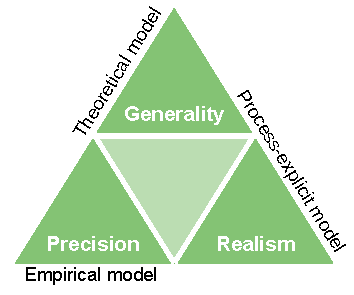
\includegraphics{0introduction/figs/levins_triangle.pdf}
\caption{\textbf{The \citet{Levins1966} triangle.}}
\label{fig:levins}
\end{figure}

Empirical models are built directly from observations and use a statistical framework to find significant relationships between observations and some explanatory variables \citep{Dormann2012}. They are particularly useful to identify patterns, within the scope of the data collected. There is usually a strong match between the model and the observations, i.e. the model describe observed phenomena with precision (\Cref{fig:levins}). However, the underlying mechanisms driving these patterns are not describe explicitly, but rather implicitly included during the creation of the model (i.e. choice of explanatory variables). \\
Theoretical models rather focus on abstract representations of ecological systems. They often try to explore and connect fundamental ecological theories \citep[][]{Chevin2010}. Even though these models are often confronted with observations to discuss the validity of the hypothesis, their primary goal is to remain general (\Cref{fig:levins}) and explain a wide variety of situations in a quite simple manner. \\
Finally, process-explicit models are of greater complexity, and explicitly simulate the processes believed to drive the observed patterns \citep{Evans2012}. The modeller choose mathematical equations to give a somewhat realistic representation of the system (\Cref{fig:levins}). These models therefore include some theoretical components, but with the primary aim of simulating specific systems. The difference with empirical models is that the structure of the model (i.e. the relationships between processes) is defined \emph{a priori}, with an explicit ecological interpretation. 

The link between experimentation and modeling varies across model classes. At some point, building a model always involves prior knowledge, derived from literature and experiments. The choice of explanatory variables in a statistical model may be motivated by previous experimental results, theoretical models rely on a coherent body of theory (some of which may have emerged from experiments), and the selection of processes and functional forms in a process-explicit model is often supported by prior research. In particular, process-explicit models heavily depend on experimental data, as most of their parameters need to be directly measured (which often limits their widespread use). The connection with experiments can also occur \emph{a posterio}: significant statistical relationships found using empirical models are often considered in a wider context  and discussed in relation to previous results (inductive reasoning; \citealp{Davi2012}).

\subsubsection{Explaining species distributions: from patterns to processes} \label{sec:approach}

One of the questions that has received a considerable amount of attention is understanding the ecological processes involved in the current geographical limits of species ranges, especially from regional to continental scales. To address it -- at least partially -- we need species distribution modeling approaches, and in particular both empirical and process-explicit models described above.

Species distribution models have been build upon the key concept of ecological niche. This concept is widespread in ecology, but we do not seek here to recount the entire scientific history of this century-old term \citep{Grinnell1917}, nor to discuss all the implications and ongoing debates. This concept will instead allow us to describe a common theoretical framework for species distribution models, and understand how they are connected despite having emerged separately.\\
The ecological niche traditionally refers to the hypervolume, in \textit{N} environmental dimensions, in which a species can maintain viable populations \citep{Hutchinson1957}. 
The fundamental niche encompasses the full range of environmental (abiotic) conditions within which a species can survive, grow, and reproduce. However, species rarely occupy their entire fundamental niche, because of some biotic interactions (competition, predation, ...) as well as dispersal limitations. These three components (abiotic, biotic, movement; \citealp{Soberon2005}) define the realized ecological niche. Thus, the potential and the realized distributions are the representations of the fundamental and the realized niche in the geographical space (i.e. the realisation of the N-dimensional hypervolume in a 2- or 3-dimensional space; \Cref{fig:glmniche}). 

\begin{figure}
\hspace*{-0.8cm}
\centering
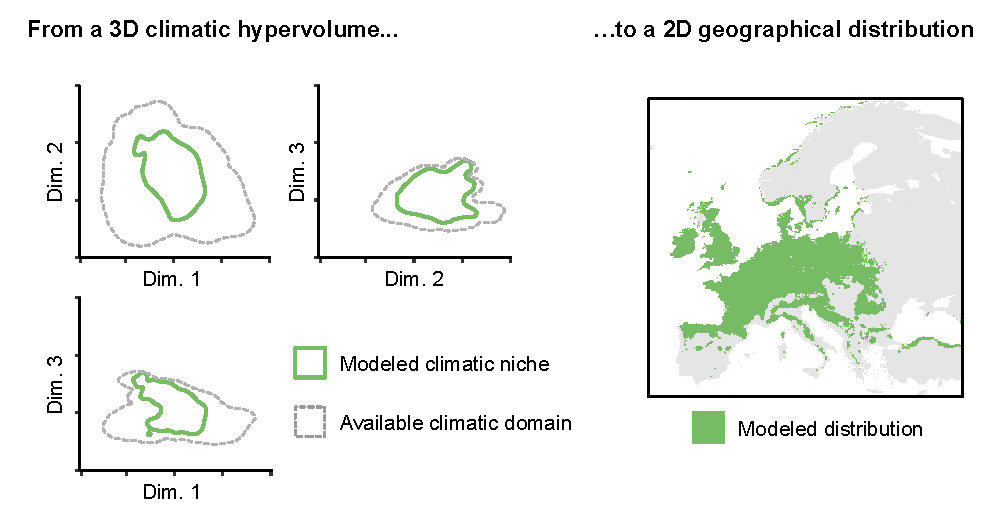
\includegraphics{0introduction/figs/glm_niche.pdf}
\caption{\textbf{Representation of a climatic niche and its equivalent distribution.} Both hypervolume and distribution corresponds to the beech distribution (\emph{F. sylvatica} L.) as simulated by a correlative GLM (see Chapter 2). The three climatic dimensions (Dim 1-3) correspond to the first three principal component axis from three-month means temperature and three-month sums of precipitation. Hypervolume contours were generated using a two-dimensional kernel density estimation.}
\label{fig:glmniche}
\end{figure}

\clearpage

The vast majority of studies seeking to understand and predict species distribution uses empirical models \citep{Dormann2012}. These models are directly derived from the ecological niche theory \citep{Guisan2000, Guisan2005}. We will call them correlative species distribution models (CSDMs) in the following -- but many other terms exist, such as environmental niche models (ENMs). They are based on statistical relationships between observed species occurrences and environmental predictors \citep{Elith2009}, mostly climatic variables (i.e. averages of monthly variables calculated over a standard 30 year period). In line with the first phytogeographic studies that identified climatic zones based on plant observations \citep{DeCandolle1820}, CSDMs take the opposite approach to project species suitable habitats from a combination of environmental variables (\Cref{fig:glmniche}). These approaches have significantly evolved, from statistical regression such as generalized linear model \citep{Thuiller2009} to artificial intelligence models utilizing dozens of variables (e.g. more than 130, \citealp{Steiner2024}). Non-climatic predictors are now also frequently used in CSDMs, such as land cover \citep{Thuiller2004, Ay2017} as well as dispersal and biotic interactions \citep{Boulangeat2012, Palacio2018}. Regardless of the explanatory variables used, the parameters can only be estimated simultaneously, as a group, when fitting the model to observations. \\
The increasing availability of high-quality, large-scale species occurrence data \citep[e.g.][]{Mauri2017}, as well as pre-formatted and easily downloadable environmental data \citep[e.g.][]{Fick2017}, has sparked a real \emph{niche modeling boom} (with more than 6000 studies between 2000 and 2020; \citealp{Araujo2019}). According to \citet{Guisan2005}, many studies make the very simplistic assumption that CSDMs model the realized species niche, given that observed distributions used for calibration are inherently constrained by biotic interactions and dispersal limitations. However, it is in reality much more nuanced, as it depends on many factors including the scale of the study. Indeed, local realized niches can be reduced without the coarse-scale pattern being affected \citep{Soberon2007}. Note also that in some cases, observed (realized) distribution may be even larger than the potential distribution, because of source-sink dynamics between populations \citep{Pulliam2000}.

Process-explicit models (PEMs) come from a different background. In parallel of the development of complex global climate models, researchers aimed at developing mechanistic models in biology, to explain the relevant physiological and physical processes at stake. Pioneer agronomists began developing PEMs as early as the 1960s (e.g. the functional relation between photosynthesis and absorbed light intensity; \citealp{Wit1965}).
The use of process-explicit crop models, however, particularly increased during the 80-90s \citep{Bouman1996}. In the same time, process-based growth and yield models were developed in forestry \citep{Botkin1972}. Applying these models at larger spatial scales than stand or landscapes to predict plant functional types or species distributions took a bit longer \citep{Sitch2003, Chuine2001} -- and it is now a hot topic \citep{Evans2016, Pilowsky2022}. 
% The development of PEMs was largely driven by the recent increased in computing power. 

\begin{figure}[h]
\hspace*{-0.8cm}
\centering
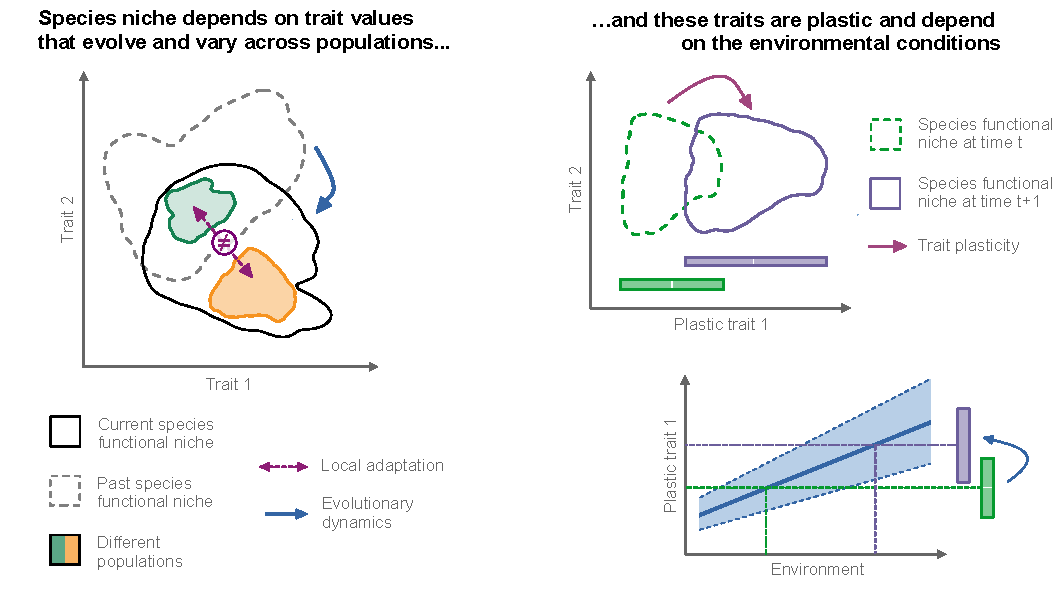
\includegraphics{0introduction/figs/functional_niche.pdf}
\caption{\textbf{The trait-based concept of ecological niche.}}
\vspace*{-0.2cm}
\label{fig:funcniche}
\end{figure}


\noindent PEMs aim at simulating the main processes that drive species functioning. They are built on explicit mathematical equations to describe causal relationships between environmental drivers and ecological responses \citep{Dormann2012}. The specific processes to include into a model are chosen according to previous theories and to the objectives of the research.
Choosing the right balance of complexity is one of the challenge of the process-based modeling: a model that is too simplistic may be unrealistic, while one that is overly complex could be highly intractable. PEMs may operate at different scales, from the gene to the ecosystem \citep{Pilowsky2022}. Within the same model, processes can also be described at different nested levels of organization and different temporal steps, depending on the model's assumptions and on our limited knowledge. For example, in the CASTANEA model \citep{Dufrene2005}, photosynthesis is simulated at the leaf level at a half-hourly timestep \citep{Farquhar1980}, whereas height growth is calculated at the end of each year for the entire tree. One of the fundamental characteristic of PEMs is that most of their parameters have a direct biological interpretation \citep{Dormann2012}. Some of these parameters can be estimated with field observations or experimental data, or are already available in the literature.  Other parameters can be calibrated using inverse modelling methods and data on the processes modeled. Classically, PEM calibration thus does not involve species occurrence data at any point -- we will call them \emph{expert} PEMs in the latter. It means that PEMs are able to simulate the potential distribution of a species independently of its observed distribution. PEM parameters are essential to allow the model to simulate realistic processes. They basically define the characteristic of populations and species -- the functional traits. In the process-explicit framework, the ecological niche can thus seen as a set of trait values rather than a set of environmental conditions \citep{Rosenzweig1987, Kearney2010}. These trait values define the interactions between a species and its environment, and may depend themselves on the environmental conditions (i.e. most traits are plastic). This \emph{functional} definition of the ecological niche thus complement the previous definition of the niche (the \emph{environmental} definition), and highlights the importance of both climatic predictors and traits in shaping species distribution (\Cref{fig:funcniche}). Moreover, a PEM focusing on a species abiotic limits should describe more closely the potential distribution (i.e. the fundamental niche) than a CSDM, as its calibration does not involve observed species and thus is theoretically not confounded by biotic and dispersal limits.

However, the distinction between correlative and process-explicit approaches is actually much more blurred and complex. All models lie somewhere on a continuum from purely statistical to purely mechanistic \citep{Korzukhin1996, Dormann2012}. On the one hand, CSDMs can be refined by explicit trait quantification \citep{BenitoGarzon2019}, demographic processes' integration \citep{Normand2014} and even by using mechanistic variables as predictors \citep{Mathewson2017}. On the other hand, most PEMs often include reasonable empirical relations, for example when knowledge is insufficient or when some processes are intentionally omitted to avoid overloading the model. Moreover, what is described as mechanistic at one level of organization could be empirical in another framework \citep{ONeill1987}. The two approaches are complementary: correlations between variables can be identified during the first stage of knowledge development, and then suggest a process-explicit representation that may produce the pattern observed. 

% The Farqhar model mentionned above was built from empirical observations 
% In many cases, empiral models are a prerequisite to the developping of process models (Korzukhin et al. (1996))

\begin{figure}[hp]
\vspace*{-0cm}
\hspace*{-0.8cm}
\centering
\begin{subcaptiongroup}
\phantomcaption\label{fig:sdmissuesA} 
\phantomcaption\label{fig:sdmissuesB}
\phantomcaption\label{fig:sdmissuesC}
\phantomcaption\label{fig:sdmissuesD}
\end{subcaptiongroup}
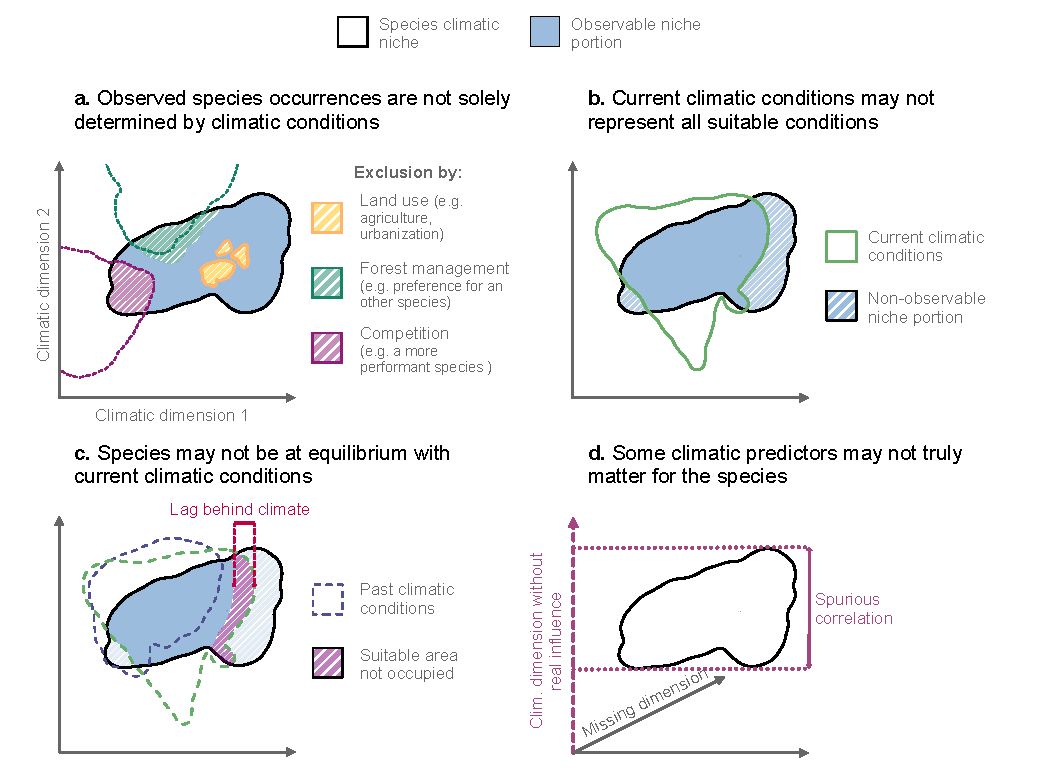
\includegraphics{0introduction/figs/sdm_issue.pdf}
\caption{\textbf{The main sources of error that can bias the results of correlative models.}}
\vspace*{-0.5cm}
\label{fig:csdmissues}
\end{figure}

\subsubsection{What can cause model error?} \label{sec:error}

Models are subject to various errors that can affect their accuracy and reliability. Both correlative and process-based models share some common sources of error. Obviously, poor-quality input data (e.g. erroneous climatic variables) can significantly alter model output. Both classes of model also frequently ignore local adaptations to specific climatic conditions and evolutionary dynamics -- but trait-based approach may provide a better framework to understand how niche may evolve across time and across populations \citep{Holt2009}. Other issues are more specific to each type of model, and it is crucial to understand them to acknowledge model uncertainties and improve model robustness.

Regarding correlative models, the bigger challenge is the incomplete niche characterization. Biases might arise from the species distribution data used during calibration \citep{BarbetMassin2010, Duputie2014, Aubry2017}. As already mentioned above, competitors may exclude species individuals from their optimal environment (\Cref{fig:sdmissuesA}). Human activies also significantly impact species occurrences, by altering species habitats (fragmentation by urbanization or agriculture; \Cref{fig:sdmissuesA}), and favoring economical important species (e.g. for forestry). The niche characterization can be incomplete because current climatic conditions do not cover the full range of conditions to which the species is pre-adapted (\citealp{Chevalier2024}; \Cref{fig:sdmissuesB}). Species may also not be in equilibrium with climate, i.e. not filling completely their range as a result of dispersal limitation of range expansion from Pleistocene refugia (\citealp{Svenning2004}; \Cref{fig:sdmissuesC}). Moreover, issues migth arise because of wrong modeling choices, leading to omission of relevant variables or inclusion of spurious correlated variables (\Cref{fig:sdmissuesD}). At a coarse scale, significant statistal relationships might indeed come from coincidence in spatial structure between explanatory variables and species distributions rather than a realistic functional relationship \citep{Bahn2007, Journe2020, Fourcade2018}.

\begin{figure}[hp]
\hspace{-1.4cm}
\centering
\begin{subcaptiongroup}
\phantomcaption\label{fig:pbmissuesA} 
\phantomcaption\label{fig:pbmissuesB}
\phantomcaption\label{fig:pbmissuesC}
\phantomcaption\label{fig:pbmissuesD}
\end{subcaptiongroup}
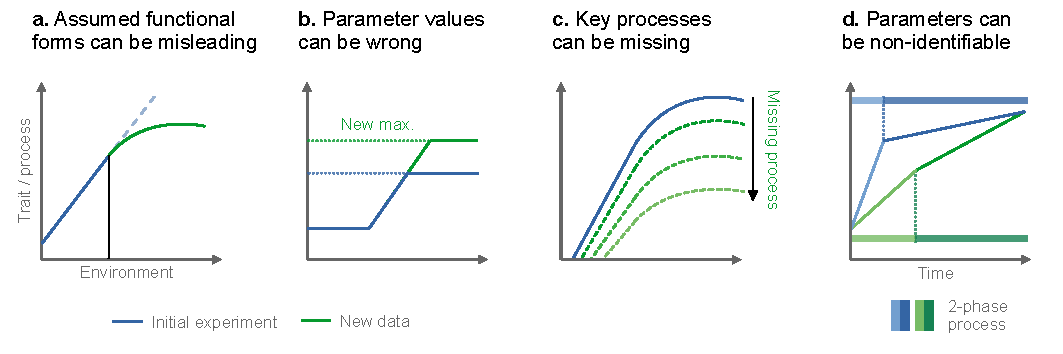
\includegraphics{0introduction/figs/pbm_issue.pdf}
\caption{\textbf{The main sources of error that can bias the results of process-explicit models.}}
\label{fig:pbmissues}
\end{figure}

Process-explicit models are also prone to a lot of errors. Modelers have to make a lot of assumptions about which processes to include, how to represent them mathematically, and how to parameterize them. All these subjective choices may introduce large errors. A process inaccurately represented -- because of a wrong mathematical assumption -- can significantly impact the output (\Cref{fig:pbmissuesA}; \citealp{Dietze2017, Wolkovich2021}). Thus, the time spent refining one process in the model can be useless if another less understood process introduces compensating errors \citep{Korzukhin1996}. Similarly, the omission of a key process may lead to erroneous dynamics (\Cref{fig:pbmissuesC}). For example, CO\textsubscript{2} effect is not always accounted for in models, even though we know it has a strong effect on PEM simulations \citep{Keenan2011a}. However, adding additional processes and complexity increases the number of parameters (\emph{parameter burden}; \citealp{Franklin2020}) and does not necessarily improve the model.
In addition, wrong parameter values are a major issue in PEMs. They can come from a lack of empirical data at a given time (\Cref{fig:pbmissuesB}). They also may arise because of compensation in modeled processes, where different parameter sets can lead to similar dynamics (\Cref{fig:pbmissuesD}; \citealp{Luo2009}), but  may generate large discrepancies when projected in different climatic conditions \citep{Chuine2016}. 

Therefore, there are multiple sources of uncertainties, and just as many possibilities of having models that cannot be reliable. In a perfect world, the niche described by a CSDM (somewhat closer to a realized niche) should be contained in the niche described by a PEM (somewhat closer to a fundamental niche) -- but this is rarely the case in reality (\Cref{fig:csdmvspbmniche}). Different PEMs can also focus on different mechanisms, and thus model different aspects of the ecological niche (e.g. growth niche vs. reproductive niche). As we deal with complex and highly interactive systems, this highlights the presence of numerous errors that we might not fully manage. Given that the future climatic conditions we face will be very different from those in which models were built and calibrated, it is critical to understand to what extent we can trust their projections.

% je peux enlever cette figure si pas utile
\begin{figure}[h]
\vspace*{-0cm}
\hspace*{0cm}
\centering
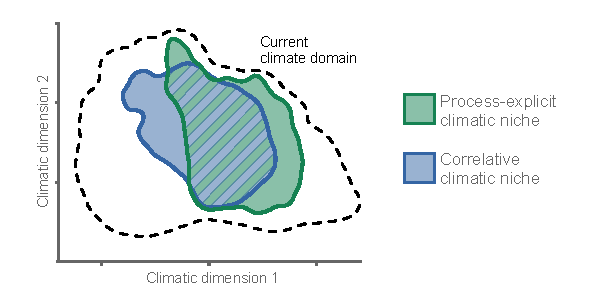
\includegraphics{0introduction/figs/csdmvspbmniche.pdf}
\caption{\textbf{Beech climatic niche as simulated by PHENOFIT and by a GLM.} The two climatic dimensions correspond to the first two principal component axis from three-month means temperature and three-month sums of precipitation (see Chapter 2). Hypervolume contours were generated using a two-dimensional kernel density estimation.}
\label{fig:csdmvspbmniche}
\end{figure}

\subsection{How to reliably forecast what the future holds?}

In the two previous parts, we have seen that:
\begin{itemize}
\item Europe has experienced major climate changes in the past, yet we are on an alarming trajectory (see this \hyperref[sec:climate]{section}); 
\item These climatic dynamics have shaped the forests we know today, which are currently threatened by rapidly shifting conditions (see this \hyperref[sec:forest]{section});
\item To gain precious insights on these threats, long-term experiments are essential but generally limited in their coverage (see this \hyperref[sec:experiment]{section});
\item Models are thus necessary to scale up to larger spatial and temporal scales (see this \hyperref[sec:model]{section});
\item There is a wide variety of models which are fundamentally different in their hypotheses and their calibration methods (see this \hyperref[sec:approach]{section});
\item And model outputs can be significantly alter by many sources of errors (see this \hyperref[sec:error]{section}).
\end{itemize}

\noindent As climate change is currently accelerating, it is really urgent to clearly and accurately determine how and why different models may provide projections with varying reliability.

\subsubsection{Into the unknown}

Warming in Europe is project to rise faster than the global mean \citep{IPCC2021}. The frequency and intensity of droughts are projected to increase \citep{Berg2016}, with strong economic impacts across the continent \citep{Naumann2021}. As a result, some ecosystems may soon surpass climatic tipping points \citep{Fewster2022}. All the effects are not yet understood: climate change may induce complex chain of events (shrinking Arctic ice, modification of ocean currents and air circulation) that induce extreme weather conditions such as persistent heat domes \citep{Oltmanns2024}. Importantly, past, current, and future emissions commit the planet to a long-term irreversible warming. Even if emissions of greenhouse gases were to stop, the climate will not quickly revert to its pre-industrial state \citep{Zickfeld2013}, and current policy decisions have strong implications for centuries to come (\Cref{fig:climatestate}; \citealp{Clark2016}).

In the face of climate change, predictive ecology is becoming a major research area \citep{Houlahan2017, Mouquet2015}. CSDMs provide alarming projections of the future of European forests \citep{Thurm2018, Dyderski2018, Chakraborty2021, Wessely2024, Mauri2022}. The number of forest tree species able to survive per square kilometer is projected to be reduced by a third by the end of the century \citep{Wessely2024}. Economically valuable species are projected to decline (34\% of Europe land could only host drought-tolerant Mediterranean forests), inducing huge economic impacts \citep{Hanewinkel2013}. However, there is a rising concern about the predictive performance of correlative approaches \citep{Bahn2007, Journe2020}. We have no guarantee that correlations are causal and will hold true in future climatic conditions, outside the range in which they were established. Climatic projections indeed indicate the appearance of novel climates in many parts of the world \citep{Williams2007, Mahony2017}, which are likely to favour the emergence of novel ecosystems \citep{Burke2019}. One must look back millions of years to find analog climatic conditions to what we can expect by the end of the century \citep{Burke2018}. As climate novelty increases, currently unobserved portions of a species niche may appear \citep{Chevalier2024}, which cannot be captured by CSDMs (as they are calibrated against observed distributions). CSDMs are known to perform poorly when projected to climatically dissimilar conditions, as species–climate correlations break down \citep{Maguire2016} -- and their accuracy is expected to decrease in the coming decades \citep{Fitzpatrick2018}. As stated by one of the anonymous reviewer of the paper by \citet{Wessely2024}, CSDM pessimistic projections may not be driven by true limiting conditions for species future growth, but rather by the fact that "\emph{the modelling approach is fundamentally flawed}" (reviewer comments visible \href{https://static-content.springer.com/esm/art%3A10.1038%2Fs41559-024-02406-8/MediaObjects/41559_2024_2406_MOESM3_ESM.pdf}{here}).

\subsubsection[Understand to predict: a tautology?]{Understand to predict: a tautology?\footnote{This title is a nod to a comment made by a PNAS editor, who thought that PEM better performance was "\emph{well established and almost tautological}" -- yet without providing any evidence of this \emph{obvious} finding.}} \label{sec:tautology}

These concerns have led to several calls to focus efforts on the development of process-explicit approaches \citep{Evans2012, Connolly2017, Urban2016, Pilowsky2022}. Their predictive power could lie in their ability to integrate all the processes determining the fundamental niche (i.e the full set of conditions where a species can maintain populations without any confounding factors such as biotic interactions). 
Hypothetically, the relationships assumed in the model are thought to be causal, because they should describe the processes that have given rise to the data we observed. These supposed cause-to-effect relationships should thus provide more robust projections in novel climatic conditions. \citet{Evans2012} draws a parallel with climate research, where long-term forecasting is done with "process-based models", as climatologists need to have a deep understanding of the underlying mechanisms that interact to be able to predict future climatic states in novel conditions (such as higher greenhouse gas concentrations). In the same spirit, ecological forecast should thus also rely on a robust understanding of these processes at stake to allow reliable projections in novel environments. This in an appealing hypothesis because PEMs are built on a more complex structure and take longer time to develop, so we can hope that these efforts are worthwhile. By their nature -- grounded in the understanding of the mechanisms -- PEMs should thus make more accurate predictions about future states. 
In some way, this could even be seen as a tautology (a statement necessarily true): if a model entails a much larger amount of \emph{a priori} knowledge and a better understanding (of the causal drivers, of the structure), shouldn't it necessarily be more performant? 
However, even though PEMs are less flexible than CSDMs, nothing prevents them from giving the right results for the wrong reasons (see \autoref{sec:error} for details). There could be a strong disparity between the ability to explain a phenomenon at the theoretical level, the ability to translate this knowledge into a well-parameterized model, and the ability to generate large-scale predictions.

Previous studies consistently found that PEMs estimate lower species extinction rates in response to climate change CSDMs \citep{Morin2009, Kearney2010, Cheaib2012, Gritti2013}. Notably, in France, major tree species such as beech and pedunculate oak could be on the brink of extinction in many regions by mid-century according to the CSDM ensemble, whereas they could maintain a broader distribution range according to PEMs \citep{Cheaib2012}. These significant discrepancies should motivate a more detailed study of the differences between the models. Yet, they are mostly ignored. One of the limitation often highlighted in the use of PEMs is that they cannot be applied easily to many species. This scientific reasoning seems somewhat hard to justify: should we stick to the correlative approach (potentially more biased) solely because the process-explicit approach (potentially more robust) is too challenging to implement? To reformulate, should we make future projections if we do not have sufficient knowledge about some species?

A new emerging avenue within the process-explicit framework is the desire to integrate the strengths of both CSDM and PEM approaches and create \emph{fitted} PEMs \citep{Dormann2012}. The general idea is to benefit from large-scale species distribution data to calibrate ecologically relevant relationships \citep{Kriticos2013, Higgins2012}, and hopefully get the best of both worlds. It is assumed that the process-explicit structure should constrain calibration outcomes, and better reproduce the distributional patterns of the species on different spatio-temporal situations than CSDM \citep{Higgins2020}. Such inverse calibration could thus help making PEMs easier to apply to a greater number of species \citep{Evans2016, Conradi2024}. However, as highlighted by \citet{Schymanski2013}, it is unclear whether this method would not simply reproduce the same issues as CSDMs, and that these fitted PEMs could just "\emph{create an illusion of predictive power by reference to their mechanistic underpinning}". One of the major advantages of this approach, in my view, is that it allows to create a middle way approach along the gradient between correlative and process-explicit approaches. CSDMs and PEMs differ by two main characteristics (see subsection \autoref{sec:model} for details): (i) statistical relationships/explicit equations with strong assumptions, and (ii) parameter estimation dependent/independent of the species distribution, i.e. what we try to model. Comparing the three types of models (CSDM, fitted PEM and expert PEM) could thus allow us to disentangle the impact of each characteristic on model performance. Yet, we have to make the effort to truly evaluate model performance under novel conditions, i.e. model transferability. This is the only way to ensure that our scientific knowledge remains valid over time \citep{Houlahan2017}.

% Confusions between the descriptive power, the explanatory power, and the predictive power \citep{Shmueli2010}: 
% - capturing the association between the dependent and independent variables
% - explaining the data-generating process with causal hypotheses
% - applying a model for the purpose of predicting new or future observations

% - Europe se réchauffe plsu vite que la moyenne\\
% - évènements extrêmes : attribution au cgt climatique\\
% - ZEC: even with zero emission: warmer world for centuries\\

\subsubsection{The difficulty to assess model transferability}

Currently, one of the prerequisite for a model to be useful for decision-making is to provide reliable projections into novel conditions \citep{Evans2012, Yates2018}. Confidence in model projections will remain limited until we can determine how well models are transferable outside the context in which they were built and calibrated -- and \emph{in fine} verify that the models are adequate for the specific purpose of ecological forecasting under climate change.

Such performance assessment has gained a lot of attention in the CSDM community \citep{Yates2018}. Numerous studies have evaluated the factors that can influence model transferability, such as the difference between species \citep{Guisan2007, Dobrowski2011, Wogan2016} or between different CSDMs \citep{Meynard2007, Valavi2022}, in particular regarding  the influence of algorithm complexity \citep{MorenoAmat2015, Bell2016, GarciaCallejas2016}. Different strategies are commonly used to try to evaluate CSDMs in the best possible way, using more or less independent datasets. The most convenient way is the cross-validation, i.e. splitting the data available in a calibration and a validation (extrapolation) set \citep{Roberts2017}. While this method can been used specifically to evaluate model transferability \citep{Wenger2012}, it is primarily the preferred method in the majority of studies for validating CSDMs. For example, in a study mentioned earlier (which project severe economic loss in the European forest sector), \citet{Hanewinkel2013} validate their CSDM framework using a 10-fold cross-validation procedure: the idea is to divide the data into 10 portions, use 9 of those portions for training the model and the last one for testing the model (and repeat the procedure 10 times, each time with a different tenth for testing). In addition to the fact that such random cross-validation strategy has been identified as inappropriate because it overestimates confidence in model predictions \citep{Roberts2017}, it may also fail to challenge modeling hypothesis with really different conditions. Other ways exist to estimate model transferability. Model can be evaluated with an independent dataset within the study area, but it does not account for different environmental conditions \citep{Guisan2007}. CSDM transferability can also be tested in different locations \citep{Randin2006, Torres2015, Sequeira2018}, for example using an invasive species to test the performance of a model calibrated only using native-range occurrences to predict the colonization dynamics \citep{Zhu2017, BarbetMassin2018}. This spatial transferability (whether using cross-validation or more independent data) is the most assessed in the literature \citep{Yates2018}. However, it is unclear whether it allows to truly evaluate the ability of CSDM to make reliable forecasts, as the effect of spatial substitution at a given time are not necessarily equivalent to the effect of temporal variations in a given location. 
Temporal transferability assessment are less common because they are more difficult to implement \citep{Yates2018}. It is usually done using historical data (over the last century; \citealp{Wogan2016, Rapacciuolo2012}), or even further in the past with paleoecological datasets \citep{MorenoAmat2015, Varela2009, Maguire2016, Veloz2012, Williams2013}. 
% cela peut être fait dans deux sens: calibrate models under climate conditions and forecasting from the past (evaluation against modern data, e.g. \citealp{Williams2013, Veloz2012}), or calibrate models with current data and hindcasting to the past (evaluation against past data, e.g. \citep{MorenoAmat2015})
All above mentioned studies have led to an awareness of the limited transferability of CSDMs under climatic conditions different from their calibration, and the fact that there may be a point beyond which sufficiently reliable projections can no longer be made (the forecast horizon; \citealp{Petchey2015}).

As noted by \citet{Yates2018}, we can expect better model transferability if the models are "\emph{grounded in well-described mechanisms}" -- such as process-explicit models. Yet, this remain mostly an hypothesis (see \autoref{sec:tautology}). 
PEM validation is indeed more tricky. 
The lower-level outputs (i.e. all the subprocesses which are modeled, such as a phenology, respiration, photosynthesis, etc.) can be validated against observations and measurements (using, in the best case, a cross-validation scheme). However, as PEM calibration does not involve species occurrence data, the ability of PEMs to simulate a species distribution cannot be evaluated using common CSDM cross-validation strategies. Up to now, PEM performance is thus mostly assessed by comparing a higher-level output (the proxy chosen to represent the species occurrence) with the species distribution \citep[e.g.][]{PetitCailleux2021}. This is far from satisfactory because we do not verify that model assumptions hold beyond current conditions. A proper and robust framework is thus lacking to compare the predictive power of PEMs and CSDMs. 

Paleoecological evidence of species range shifts in response to past climate change offer an unique opportunity to assess model transferability \citep{Maguire2015}, and in particular whether there is a real increase in predictive accuracy achieved by moving from a statistical approach to a more process-explicit one. However, it can be quite challenging to apply CSDMs and PEMs to past climates. \\
First, running these models necessitates input climatic data. One approach involves reconstructing bioclimatic variables from fossil data \citep{CruzSilva2023}, though this may introduce a circularity if the same fossil data are later used to evaluate models. An other possibility is to use simple climate model (with a simpler representation of physical processes and a coarser-resolution than state-of-the-art global climate models) to generate transient simulations of past climate change \citep{Goosse2010}. Nevertheless, the computational challenge of producing global time series using fully coupled complex climate models can be overcome. One can generate model output at 1000-year intervals over the period, with different forcing conditions (\emph{snapshot} approach), while still considering millennial-scale fluctuations that may significantly impact ecosystems \citep{Armstrong2019}. The output from such simulations (including variables such as cloudiness) then allows for a more robust stochastic generation of daily climatic variables using weather generators \citep{Sommer2017} -- an essential step if we want to use PEMs. \\
Evaluating models in the past also requires proxies for species past distributions. 
Fossil pollen is the most important source of data. Recent efforts to compile and curate these data at a global scale now facilitate their use \citep{Fyfe2009, Williams2018}. One of the challenge is to estimate the age of these fossil pollen (the chronology), which is done using age-depth models based on control points for which we have a dating \citep{MorenoAmat2017}. These chronologies must then be standardized across the different records \citep{Herzschuh2022}. Fossil pollen data may also be completed with other sources, such as ancient DNA \citep{Dalen2007} or plant macrofossils \citep{Cordova2009}. There are however numerous limitations inherent to the use of these paleodata \citep{MorenoAmat2017}. Pollen data coverage is restricted to the locations where sedimentary cores have been sampled, with a bias towards sites with favorable conditions for fossil conservation \citep{Varela2011}. Moreover, pollen morphological features used to identify fossils are often shared by several taxa, which most of the time prevents an identification beyond the genus level \citep{MorenoAmat2017}. This can be a significant issue when there are many species within the same genus in a particular area (e.g. \emph{Pinus} in the Mediterranean region). Finally, there is not a direct link between fossil assemblages and past vegetation. All species are indeed not equally represented, because of different pollen production and  dispersion across taxa \citep{Goring2013}, and the absence of pollen may not imply the absence of the source plant \citep{Hicks2006}.\\
Despite these challenges, if models are evaluated using consistent data (similar climatic and fossil datasets), their relative performance can still be assessed, keeping in mind all the limitations and the particular context of this performance comparison.

\subsection{Objectives and plan}

Experts are concerned by the uncertainties on the impact of long-term climate and disturbance trajectories on forests \citep{Buma2024}. This highlights that it is urgent to clearly and accurately determine the relative robustness of the different types of models that intend to provide projections of species distributions in the near future, and to identify the causes of their robustness or lack of robustness. Management strategies that will help forests to adapt will be critical, and there is a crucial need for reliable projections to support evidence-based decision making, with a robust quantification of uncertainties. Our general objective with this PhD work was thus to assess the robustness and uncertainty of projections of the future distribution of forest trees. To achieve this, the work is structured into the four following chapters. % (\Cref{fig:timeline}).

\begin{figure}[H]
\vspace*{-0.5cm}
\centering
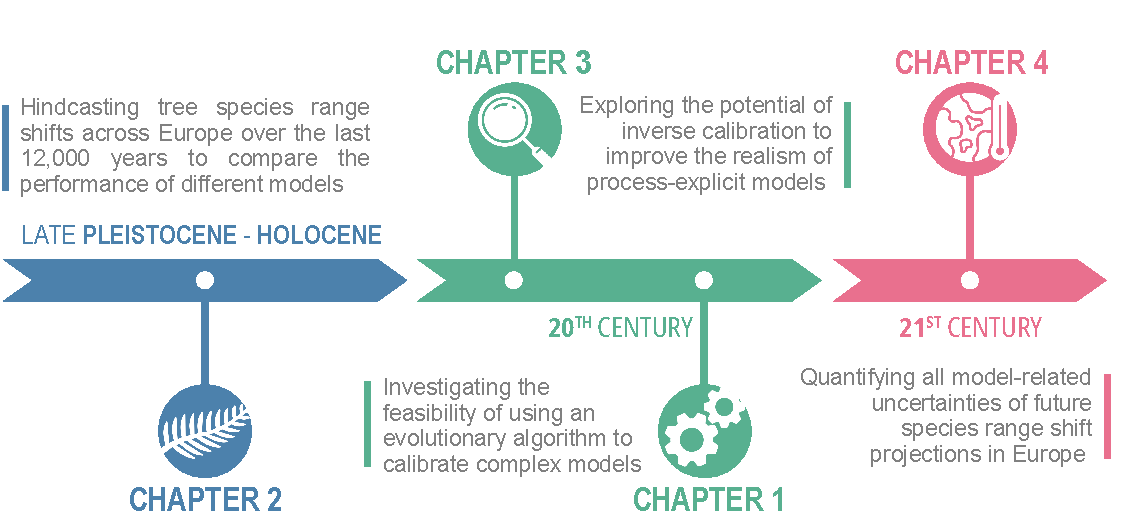
\includegraphics{0introduction/figs/timeline.pdf}
%\caption*{\textbf{The timeline of this PhD thesis.}}
\vspace*{-5cm}
\label{fig:timeline}
\end{figure}

\clearpage

\textbf{Chapter 1: Applying an efficient optimization algorithm to calibrate process-explicit models using species occurrence data}

\vspace*{0.1cm}

\noindent The first step of this PhD thesis was to explore whether it was feasible to calibrated complex PEMs with numerous parameters using the same data as CSDMs. To this aim, we adapted a robust optimization algorithm (covariance matrix adaptation evolution strategy), which has never been used in ecology to our knowledge. \\
The main goals of this chapter were: \\
(i) to explore the feasibility of inverse calibration\\
(ii) to develop an hybrid modeling approach (fitted PEMs, with process-explicit equations and calibrated using species occurrence data) in order to encompass the full spectrum of models in the next chapter

\vspace*{0.5cm}

\textbf{Chapter 2: Making a comprehensive comparison of the ability of various modeling approaches to hindcast tree species range shifts over the last 12,000 years}

\vspace*{0.1cm}

\noindent The second step of this PhD thesis was to provide for the first time a simultaneous evaluation of the transferability of CSDMs, fitted PEMs and expert PEMs in very different climatic conditions -- taking account the migration. One of the challenges was to process paleoclimatic data, and in particular to generate daily variables required by the PEMs. On the one hand, the comparison between CSDM and fitted/expert PEM projections allowed us to test for the hypothesis that model robustness is conveyed by the process-explicit relationships described in the PEM. On the other hand, the comparison between fitted PEMs and expert PEMs allowed us to test for the hypothesis that model robustness is conveyed by the fact that parameters values are not calibrated using species occurrence data.

\vspace*{0.5cm}

\textbf{Chapter 3: Investigating to what extent inverse calibration can help improving process-explicit models}

\vspace*{0.1cm}

\noindent While chapter 2 provided a large-scale and long-term model evaluation, we wanted in this chapter to understand more thoroughly to what extent inverse calibration may help foster the use of PEMs for a larger number of species. In particular, we investigated whether PEM structure would sufficiently constrain the calibration process, and to what extent fitted PEMs may simulate realistic processes.

\vspace*{0.5cm}

\textbf{Chapter 4: Capturing the full breadth of uncertainties that are relevant to assess how climate change will affect forests across Europe}

\vspace*{0.1cm}

\noindent Finally, the last objective of this PhD thesis was to produce projections of species range shifts in different future climate scenarios with associated uncertainties. We wanted to quantify the different sources of uncertainties and their relative importance. In particular, we investigated how ignoring the uncertainties related to the different SDM types could impact forest management in Europe.

\newpage
\
\newpage